% !TEX root = ../EntropicNumeric.tex 


\section{Applications}
\label{sec_applications}

Throughout this Section, we detail how to use the scaling iterations~\eqref{eq-scaling-iterates} for solving the problems discussed in Section \ref{sec-ot-like}. We first analyze the properties of the functionals on marginals $F_i$, then we derive the iterations in a continuous setting, and finally show numerical experiments. We extend the definition of the operator $\sproxdiv$ (defined in \eqref{eq_proxdiv} in the discrete setting) to the continuous setting as follows: for $s\in \Lun(X)$, $u \in \Linf(X)$ and $\epsilon>0$
\eql{
\label{eq_proxdivbis}
\sproxdiv_{F}(s,u,\epsilon) = \prox^{\KL}_{F/\epsilon}(s\, e^{-\frac{u}{\epsilon}} ) /s
}
with the convention $0/0=0$. Moreover, in order to avoid the heavy notation $\Divergm_\phi(a\d x|b \d x)$, we denote by straight letters the divergences between functions, i.e. for $a,b$ measurable nonnegative functions on $X$ and $\varphi$ a nonnegative entropy function (see Definition \ref{def_entropy}):
\eql{\label{eq_divergencefunctions}
 \Diverg_\phi(a|b) \eqdef \int_X \ol{\Diverg}_\phi(a(x)|b(x)) \d x
 \qwithq
 \ol{\Diverg}_\phi(a|b) = 
 \begin{cases}
 b\cdot \phi(a/b) & \text{if $b>0$}\\
 a\cdot \varphi'_\infty & \text{otherwise}\, .
 \end{cases}
}
with the convention $0\times \infty=0$. Some properties of these divergences between functions are studied in Appendix \ref{sec:ApxDivergences}.


All reported runtimes were obtained with an implementation in Julia, on a standard laptop with CPU clock rate $2.5$ GHz.

%%%%%%%%%%%%%%%%%%%%%%%%%%%%%%%%%%%%%%%%%%%%%%%
\subsection{Balanced and Unbalanced Optimal Transport}
\label{sec_appli_UOT}

\paragraph{Derivation of the algorithm.}

The basic framework of classical and unbalanced optimal transport has been recalled in Sections \ref{subsec_balanced} and \ref{subsec_unbalanced}. Assume that we are given marginals $\mu\in \Mm_+(X)$, $\nu \in \Mm_+(\nu)$ and a cost function $c:X\times Y \to \RR \cup \{\infty\}$. By defining $p = \d \mu /\d x$ and $q=\d \nu /\d y$, the marginal functionals involved in the regularized problem are
\eql{\label{eq_UOT}
F_1(s_1) = \Diverg_{\phi_1}(s_1 | p )
\qandq
F_2(s_2) = \Diverg_{\phi_2}(s_2  | q )\, .
}
as in \eqref{eq_divergencefunctions} above. As shown in Appendix \ref{sec:ApxDivergences}, if $\phi$ is a nonnegative entropy function (Definition \ref{def_entropy}) then $F_1$ and $F_2$ are admissible integral functionals (Definition \ref{def_integralfunctional}). In order to compute the associated $\proxdiv$ operator, let us apply Proposition \ref{prop_proxKLcont} in this precise case.
%
\begin{proposition}
\label{prop_UOTprox}
Let $\phi$ be a nonnegative entropy function and $(s,p)\in \Lun_+(X)^2$ such that $0\in \dom \phi$ or $s(x)=0 \Rightarrow p(x)=0$ a.e. Let $F(s)=\Diverg_{\phi}(s | p )$. Then $\prox^{\KL}_{F/\epsilon}(s)$ is not empty and is the singleton�$s^\star$ satisfying for a.e. $x\in X$,
\eq{
\begin{cases}
0 = s^\star(x) & \text{if $s(x)=0$,}\\
0 = \epsilon \log(s^\star(x)/s(x)) + \phi'_\infty & \text{if $p(x)=0$ and $s(x)>0$,}\\
0 \in \epsilon \log(s^\star(x)/s(x)) + \partial \phi(s^\star(x)/p(x)) & \text{otherwise.}
\end{cases}
}
\end{proposition}
\begin{proof}
It is the pointwise optimality conditions associated to Proposition \ref{prop_proxKLcont}.
\end{proof}
%
This formula allows to compute explicitly the $\proxdiv$ operators of the examples introduced in Section \ref{sec_divergencefunc}, as listed in Table \ref{table_proximalexplicit}. These entropy functions as well as the associated $\proxdiv$ operators are displayed on Figure \ref{fig_fdiv}. Note that, in Table~\ref{table_proximalexplicit} the first line corresponds to standard Sinkhorn iterations and these iterations are recovered in the second and third line by letting $\la\to + \infty$ and by setting $\alpha=\beta=1$ in the fourth line.
%
In the context of the log-domain stabilization (Section \ref{sec:LogDomain}), all four $\proxdiv$ operators remain stable in the limit of small $\epsilon$: either $\proxdiv$ is independent of $u$, only a regularized exponential $e^{-u/(\lambda + \epsilon)}$ must be evaluated, or extreme values are cut off by thresholding.


\begin{table}[h] \centering
%\arraystretch
\begin{tabular}{@{}rcrcr@{}}\toprule
$F$
&& $\proxKL_{F/\epsilon}(s)$ &&$ \proxdiv_F(s,u,\epsilon) $\\ \midrule
$\iota_{\{=\}}(\cdot | p) $
&& $p$ 
&& $p/s$ 
\\ \addlinespace
$\lambda \KL(\cdot | p)  $
&& $s^{\frac{\epsilon}{\epsilon+\lambda}} \cdot p^{\frac{\lambda}{\epsilon+\lambda}}$
&& $\left( p/s \right)^{\frac{\lambda}{\lambda+\epsilon}} \cdot e^{-u/(\lambda+\epsilon)}$ \\ \addlinespace
$\lambda \TV(\cdot | p) $
&& $\min \left\{ s \cdot e^{\frac{\lambda}{\epsilon}}, \max \left\{ s \cdot e^{-\frac{\lambda}{\epsilon}}, p \right\} \right\}$
&& $\min \left\{ e^{\frac{\lambda-u}{\epsilon}}, \max \left\{ e^{-\frac{\lambda+u}{\epsilon}}, p/s \right\} \right\}$  
\\ \addlinespace
$\RG_{[\alpha,\beta]} $
&& $ \min \left\{ \beta \, p, \max \left\{ \alpha\, p, s \right\} \right\} $
&& $\min \left\{ {\beta \, p}/{s}, \max \left\{ {\alpha\, p}/{s}, e^{-u/\epsilon} \right\} \right\}$
\\ \addlinespace \bottomrule
\end{tabular}
\caption{Some divergence functionals and the associated $\prox$ and $\proxdiv$ operators for functions $s$ and $u$ defined on $X$. All operators are acting pointwise and $\lambda>0$, $0\leq\alpha\leq\beta$ are real parameters (see Section \ref{sec_divergencefunc} for the definitions).}
\label{table_proximalexplicit}
\end{table}
%
\begin{figure}
\centering
\begin{subfigure}{0.45\linewidth} 
\centering
 \resizebox{1.\linewidth}{!}{
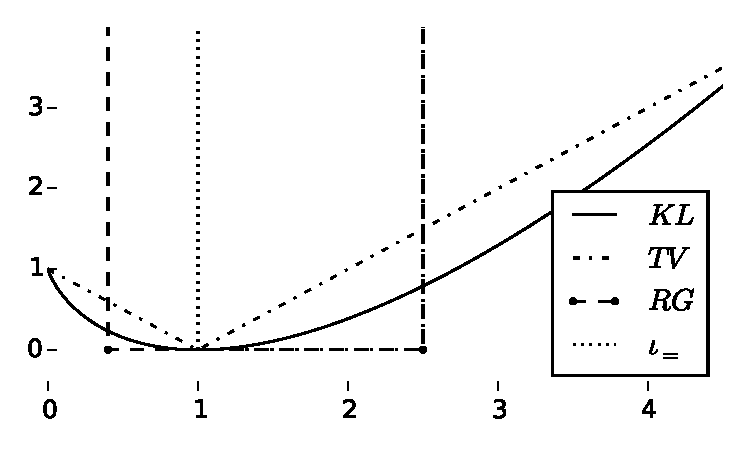
\includegraphics[clip,trim=0cm 0cm 0cm 0cm]{fdivergences.pdf}
}
\caption{Graph of the entropy functions $\varphi$ used to define the divergences in the legend.}
\end{subfigure}%
 \centering
 \qquad
\begin{subfigure}{0.45\linewidth} 
\centering
 \resizebox{1.\linewidth}{!}{
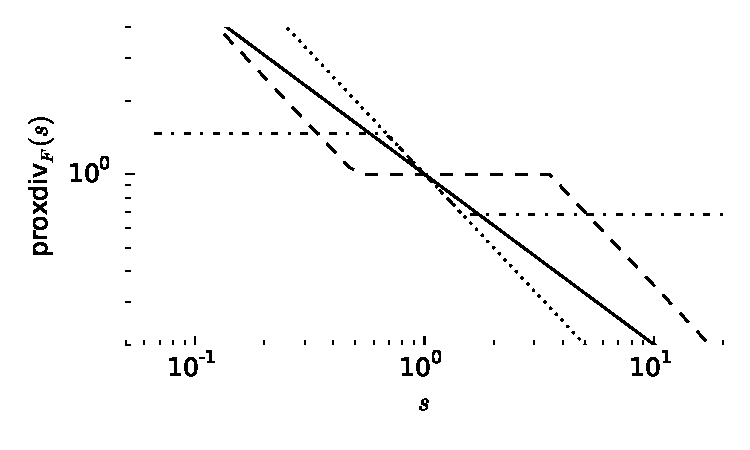
\includegraphics[clip,trim=0cm 0cm 0cm 0cm]{proxs.pdf}
}
\caption{Operator $\proxdiv_F$ associated to these divergence functions, for $p=1$, $u=0$ and varying $s\in \RR$ (in $\log$ scale)}
\end{subfigure}%
\caption{Divergences and $\proxdiv$ operators for the examples of Table \ref{table_proximalexplicit}}
\label{fig_fdiv}
\end{figure}

%%%%%%%%%%%%%%%%%%%%%%%

%\begin{remark}[Multiple Proximal Steps for Balanced Optimal Transport]
%	\label{rem:MultipleProxSteps}
%	In Section \ref{subsec:EntropicRegularization} the interpretation of the regularized problem as a proximal step w.r.t.\ the Kullback-Leibler divergence was discussed. For balanced optimal transport it turns out that $\ell$ steps with stepsize $\epsilon$ yield the same result as one step with stepsize $\epsilon/\ell$.
%	
%	For simplicity, let $X$ and $Y$ be finite spaces with fully supported probability measures $\mu$ and $\nu$, let $c$ be a finite cost function on $X \times Y$ and consider the functional $\mathcal{J}(\gamma) = \langle c, \gamma \rangle
%	 + \iota_{\{=\}}(P^X_\# \gamma | \mu) 
%	 + \iota_{\{=\}}(P^Y_\# \gamma | \nu)$.
%	 Choose a fully supported reference measure $\gamma_0 \in \Mm_+(X \times Y)$. Let $\epsilon_1$, $\epsilon_2 > 0$ be two regularization parameters and set $\gamma_{1} \eqdef \prox^{\KL}_{\mathcal{J}/{\epsilon_1}}(\gamma_0)$, $\gamma_{2} \eqdef \prox^{\KL}_{\mathcal{J}/{\epsilon_2}}(\gamma_1)$.
%	 Then we find that $\gamma_1$ can be written as $\gamma_1(x,y) = a(x)\,b(y)\,K_1(x,y)\,\gamma_0(x,y)$ with $K_1(x,y) = \exp(-c(x,y)/\epsilon_1)$, for two functions $a$ and $b$.
%	 The functional to determine $\gamma_2$ is consequently given by...
%\end{remark}

%%%%%%%%%%%%%%%%%%%%%%%%%%%%%%%%%%%%%%%%%%%%%%%%
%%%%%%%%%%%%%%%%%%%%%%%%%%%%%%%%%%%%%%%%%%%%%%%%

\paragraph{Numerical examples for $X=[0,1]$.}

Let $X=Y$ be the discretization of the interval $[0,1]$ into $I=J=1000$ uniform samples and $\mathbf{\d x} = \mathbf{\d y} = \frac{1}{I} \ones_I$ (the discretized Lebesgue measure). Let $\mathbf{p}$, $\mathbf{q}$ be the (discrete) marginals displayed on Figures \ref{fig_marg1d_p}-\ref{fig_marg1d_q}. We solve the discrete entropic regularized problem \eqref{eq_primal_discr} using the stabilized scaling Algorithm \ref{algo_scaling_stabilized} for marginal functions $F_i$ of the form \eqref{eq_UOT} with several choices of divergences listed in Figure \ref{fig_1Dmarginals}. The algorithm was stopped after $10^3$ iterations with a runtime of approximately $30$ seconds. 

For the optimal solution $\mathbf{R}\in \RR^{I\times J}$, obtained after convergence, Figure \ref{fig_1Dmarginals} displays its projections�$\mathbf{R}\, \mathbf{\d y}$ and $\transp{\mathbf{R}}\, \mathbf{\d x}$ on the domain $X$ and Figure \ref{fig_1Dplans} illustrates the entries of $\mathbf{R}$ which are greater than $10^{-10}$. Thanks to the stabilization of Algorithm \ref{algo_scaling_stabilized}, the parameter $\epsilon$ could be made extremely small, until the plan is quasi-deterministic. Here we set it to $\epsilon=10^{-7}$ for the support to be clearly visible on Figure \ref{fig_1Dplans}. Remark that for the $\TV$ case (orange support), the straigth segments correspond to a density of $1$ on the diagonal: this is the plan with minimal entropy among the (non-unique) optimal plans, in accordance to Proposition \ref{prop_converg_regul}.

Figure \ref{fig_convergenceUOT} displays the primal-dual gap $\eqref{eq-general-regul-KL}-\eqref{eq-dual-pbm}$ as a function of the iteration $\ell$ when running Algorithm \ref{algo_scaling_discrete} for solving unbalanced optimal transport problems with $\epsilon=0.01$. The marginals are the same as shown on Figures \ref{fig_marg1d_p}-\ref{fig_marg1d_q}, the cost is quadratic and terms in the primal or dual functional which are indicator of convex sets are replaced by an exponential function of the distance to that set. The discretization is $I=J=500$ except for the thin black line where $I=J=1000$. This plot leads to 3 observations which generalize the conclusion of Theorem \ref{th_convergenceKL}: (i) convergence is linear in all cases (ii) convergence is faster when the divergences are multiplied by a small weight (iii) convergence speed is insensitive to dimension of the problem. 
%
%The following list gives the parameters of the numerical experiments as well as the name they are given in the figures (for all of them $I_{f_1}=I_{f_2}=\Diverg_\phi$ with the given $\phi$):
%\begin{itemize}
%\item Optimal transport: $c(x,y)=|x-y|^2$ and $\varphi = \iota_{\{1\}}$;
%\item Optimal partial transport : $c(x,y)=|x-y|^2$ and $\varphi = 0.05 \times |x-1|$; 
%\item Gaussian-Hellinger-I: $c(x,y)=|x-y|^2$ and $\varphi = 0.5 \times\phi_{\KL}$;
%\item Gaussian Hellinger-II: $c(x,y)=|x-y|^2$ and $\varphi = 0.1 \times \phi_{\KL}$;
%\item Range optimal transport: $c(x,y)=|x-y|^2$ and $\varphi = 0.1 \times \iota_{0.7 \leq x \leq 1.2}$; 
%\item $\WassF$: cost as in \eqref{logcost} and $\varphi = \phi_{\KL}$;
%\end{itemize}
%
%%%%%%%%%%%%%%%%%%%%%%%%%%%%%%%%%%%%%%%%%%%%%%%%%%
\begin{figure}
 \centering
\begin{subfigure}{.5\linewidth}
\centering
 \resizebox{1.\linewidth}{!}{
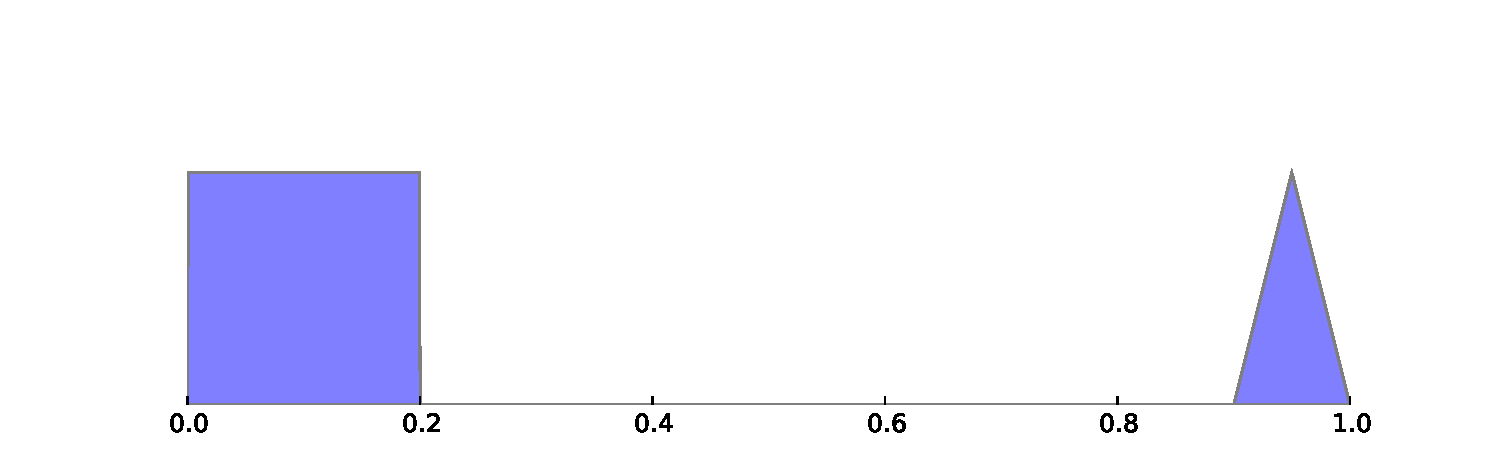
\includegraphics[clip,trim=0cm 0cm 0cm 0cm]{margs1d_p}
}%
\caption{Marginal $p$}\label{fig_marg1d_p}
\end{subfigure}%
 \begin{subfigure}{.5\linewidth}
\centering
 \resizebox{1.\linewidth}{!}{
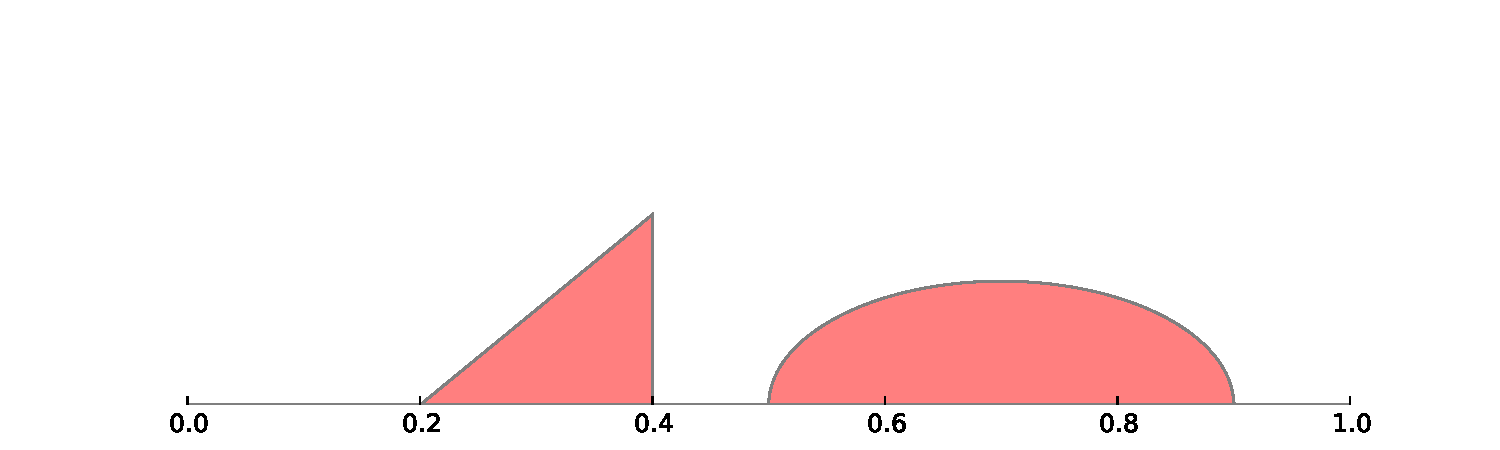
\includegraphics[clip,trim=0cm 0cm 0cm 0cm]{margs1d_q}
}%
\caption{Marginal $q$}\label{fig_marg1d_q}
\end{subfigure}
 %
\begin{subfigure}{0.5\linewidth} 
\centering
 \resizebox{1.\linewidth}{!}{
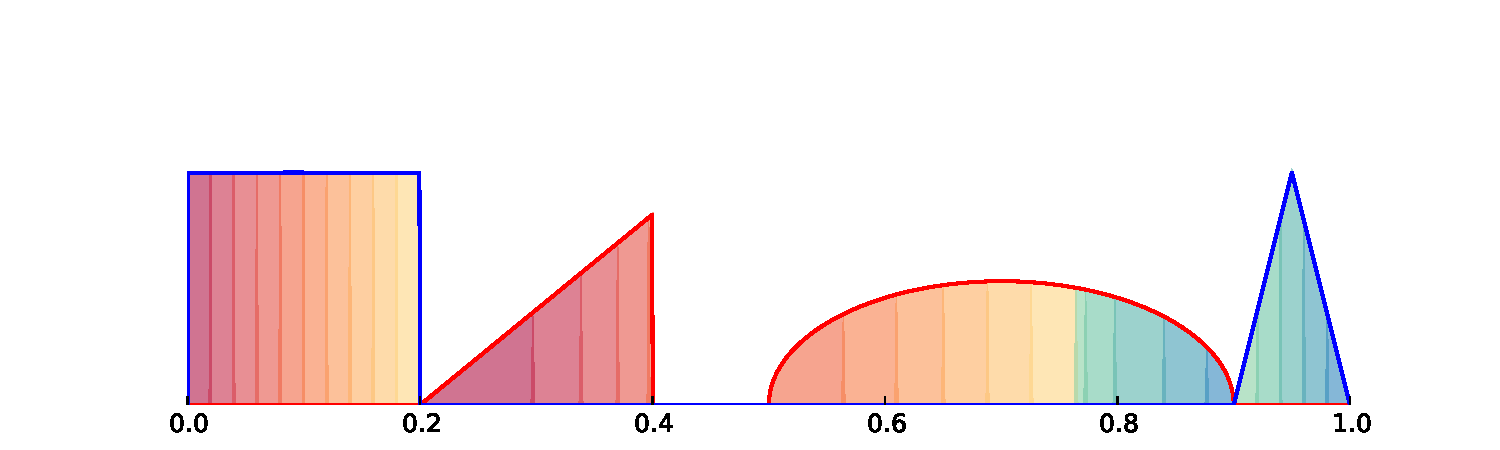
\includegraphics[clip,trim=0cm 0cm 0cm 0cm]{margs1d_OT}
}
\caption{$\iota_{\{=\}}$ (classical OT)}
\end{subfigure}%
\begin{subfigure}{0.5\linewidth} 
\centering
 \resizebox{1.\linewidth}{!}{
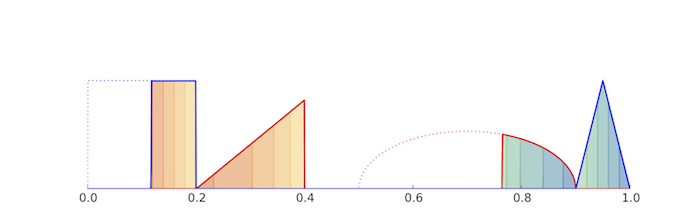
\includegraphics[clip,trim=0cm 0cm 0cm 0cm]{margs1d_TV}
}
\caption{$0.05\times \TV$}
\end{subfigure}
\begin{subfigure}{0.5\linewidth} 
\centering
 \resizebox{1.\linewidth}{!}{
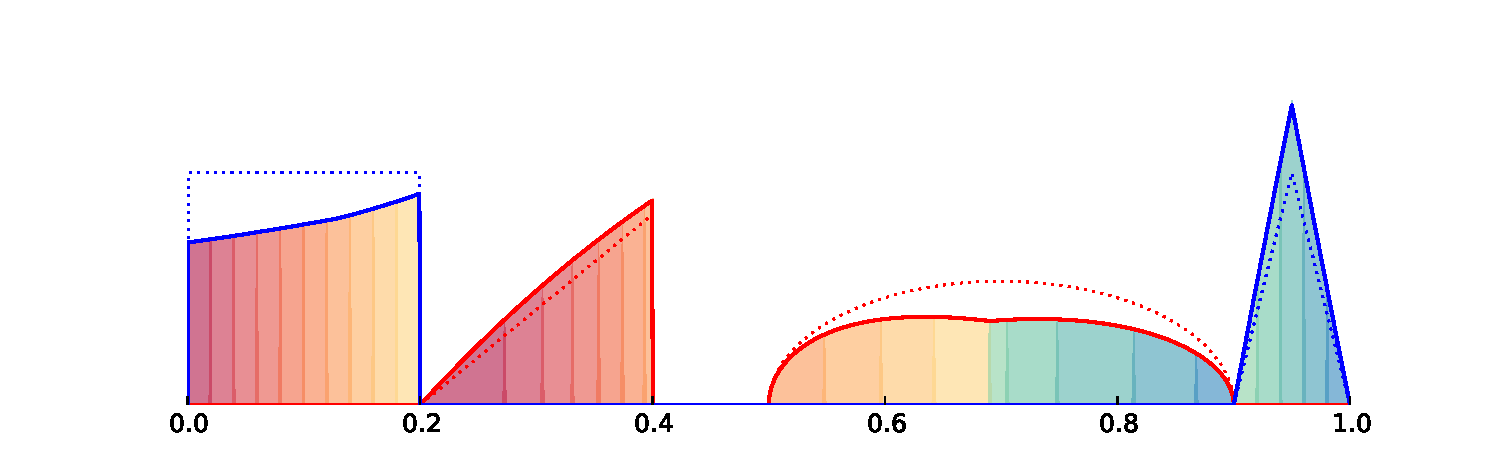
\includegraphics[clip,trim=0cm 0cm 0cm 0cm]{margs1d_KLa}
}%
\caption{$0.5\times \KL$}
\end{subfigure}%
\begin{subfigure}{0.5\linewidth} 
\centering
 \resizebox{1.\linewidth}{!}{
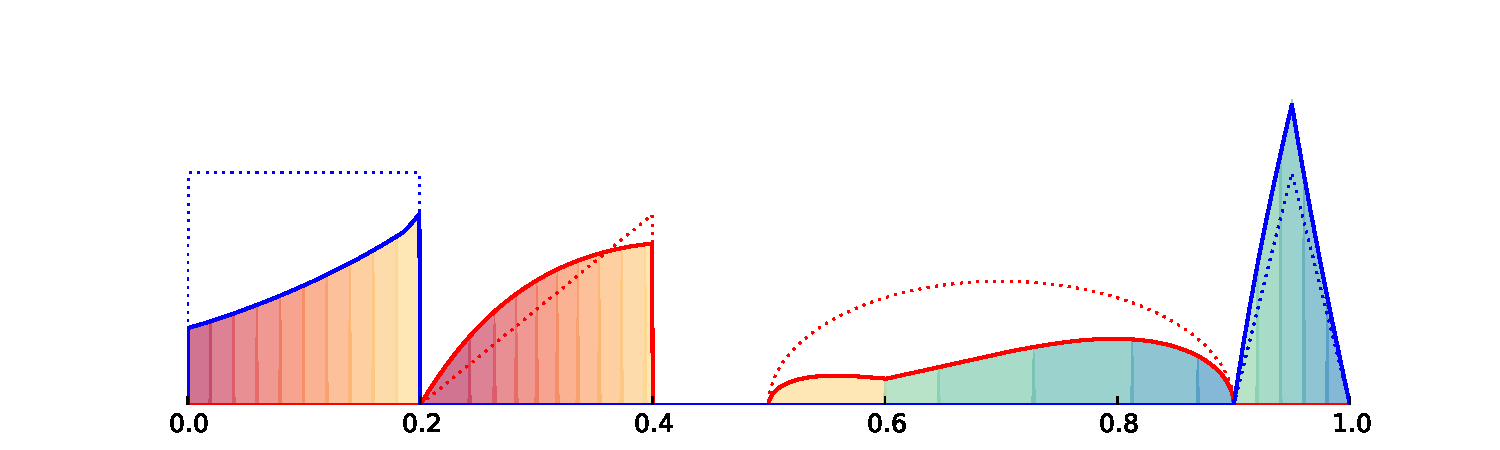
\includegraphics[clip,trim=0cm 0cm 0cm 0cm]{margs1d_KLb}
}
\caption{$0.1\times \KL$}
\end{subfigure}
\begin{subfigure}{0.5\linewidth} 
\centering
 \resizebox{1.\linewidth}{!}{
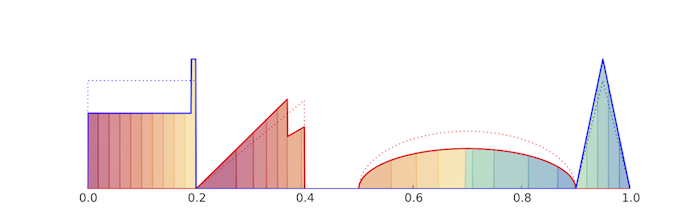
\includegraphics[clip,trim=0cm 0cm 0cm 0cm]{margs1d_RG}
}%
\caption{$\RG_{[0.7,\, 1.2]}$}
\end{subfigure}%
\begin{subfigure}{0.5\linewidth} 
\centering
 \resizebox{1.\linewidth}{!}{
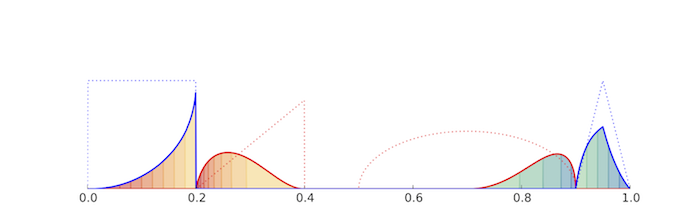
\includegraphics[clip,trim=0cm 0cm 0cm 0cm]{margs1d_WF}
}%
\caption{$\WassF$ (with cut locus at $0.2$)}
\end{subfigure}%
\caption{(a)-(b) Input marginals. (c)-(h) Marginals of the optimal plan $\mathbf{R}$ displayed together for several divergences (specified in the caption). The color shows the location of the same subset of mass before and after transportation. The cost is the quadratic cost $c(x,y)=|y-x|^2$ except for (f) which is a computation of the optimal plan for $\WF$ that is $F_1=F_2=\KL$ and $c$ as in \eqref{logcost} (with a spatial rescaling so that $c(x,y)=\infty \Leftrightarrow |y-x|\geq0.2$).}
\label{fig_1Dmarginals}
\end{figure}
%%%%%%%%%%%%%%%%%%%%%%%%%%%%%%%%%%%%%%%%%%%%%%%%%%
\begin{figure}
 \centering
 \resizebox{.40\linewidth}{!}{
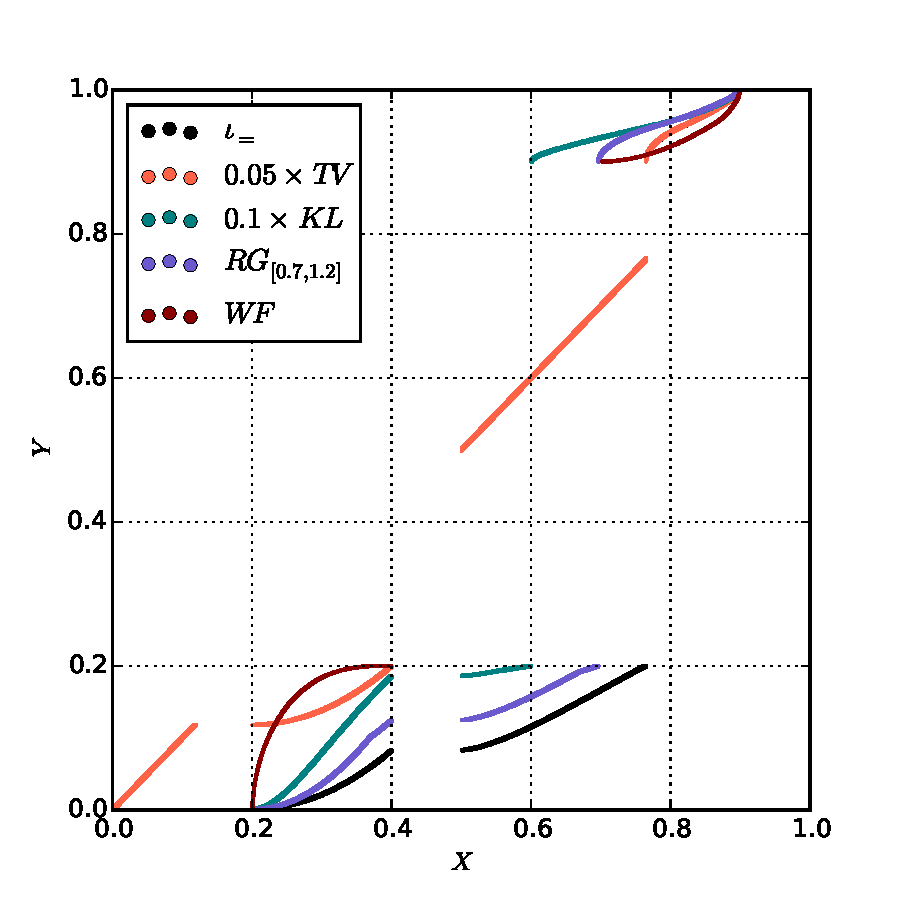
\includegraphics[clip,trim=0cm 0cm 0cm 0cm]{plan1d.pdf}
}%
\caption{Support of the optimal plans $\enscond{(x_i,y_j)}{\mathbf{R}_{i,j}>10^{-10}}$ for all the examples displayed on Figure \ref{fig_1Dmarginals}, except (e). Orange and black are superimposed at the top.}
\label{fig_1Dplans}
\end{figure}
%%%%%%%%%%%%%%%%%%%%%%%%%%%%%%%%%%%%%%%%%%%%%%%%%
\begin{figure}
\centering
 \resizebox{.7\linewidth}{!}{
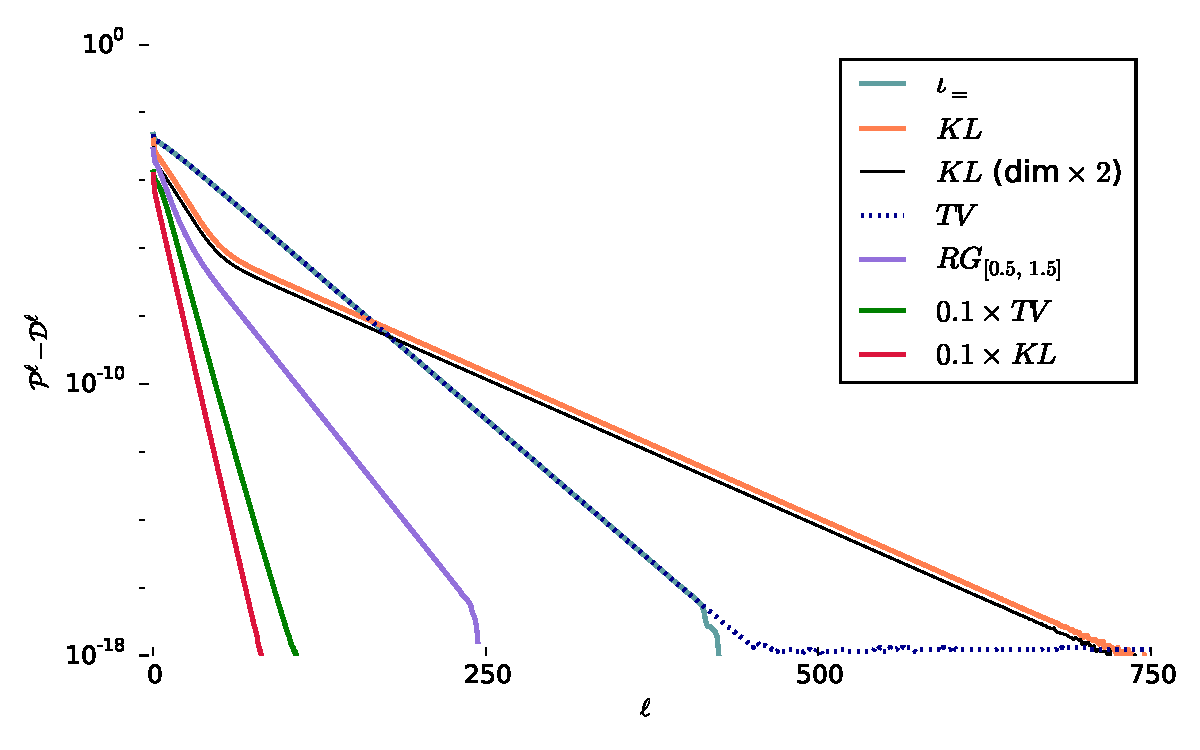
\includegraphics[clip,trim=0cm 0cm 0cm 0cm]{convergenceplain2}
}
\caption{Primal dual gap as a function of the iterations for Algorithm \ref{algo_scaling_discrete} applied to unbalanced optimal transport problems.}
\label{fig_convergenceUOT}
\end{figure}
%%%%%%%%%%%%%%%%%%%%%%%%%%%%%%%%%%%%%%%%%%%%%%%%%%
\paragraph{Numerical examples for $X=Y=[0,1]^2$.}

Let $X=Y$ be the discretization of the $2$-dimensional domain $[0,1]^2$ into $I=J=200\times 200$ uniform samples and $\mathbf{\d x} = \mathbf{\d y} $ be the discrete Lebesgue measures. Let $p$, $q$ be the densities displayed together on Figure \ref{fig_marg2d} and $c$ be the quadratic cost�$c(x,y)=|y-x|^2$. We solve the discrete entropic regularized problem \eqref{eq_primal_discr} using Algorithm \ref{algo_scaling_discrete} for several unbalanced optimal transport problems. 
%
We apply the ``separable kernel'' method (see Section \ref{sec_implementation}) to accelerate the algorithm. Since this cannot be combined with the log-stabilization, the regularization parameter $\epsilon$ has been fixed to the rather high value $\epsilon=10^{-4}$ in order to avoid numerical issues.
%
Figure \ref{fig_2Dmarginals} shows the marginals of the optimal coupling $\mathbf{R}$ and Figure \ref{fig_2Dplans} illustrates the resulting transport plan: points with the same color correspond roughly to the same mass particle before and after transport. %(more precisely, the color represents, on the support of $p$ , the horizontal coordinate and, on the support of $q$, the horizontal coordinate of $T^{-1}(x,y)$  where $T$ is the transport map associated to $R$). \todo{B: to me the more precise explanation is more confusing than it helps, also it mentions a map $T$ which we don't introduce, etc. I would simply delete it.}
%
The algorithm was stopped after $10^3$ iterations and the running time was of $35$ seconds approximately.
%

%%%%%%%%%%%%%%%%%%%%%%%%%%%%%%%%%%%%%%%%%%%%%
\begin{figure}
 \centering
 %
\begin{subfigure}{0.22\linewidth} 
\centering
 \resizebox{1.\linewidth}{!}{

\includegraphics[clip,trim=0cm 0cm 0cm 0cm]{margs2d}
}
\caption{$p$ and $q$}\label{fig_marg2d}
\end{subfigure}%
\begin{subfigure}{0.22\linewidth} 
\centering
 \resizebox{1.\linewidth}{!}{

\includegraphics[clip,trim=0cm 0cm 0cm 0cm]{margs2d_KLb}
}%
\caption{\small{$ 0.1\! \times\! \KL$}}
\end{subfigure}
\begin{subfigure}{0.22\linewidth} 
\centering
 \resizebox{1.\linewidth}{!}{

\includegraphics[clip,trim=0cm 0cm 0cm 0cm]{margs2d_RG}
}%
\caption{\small{$\RG_{[0.7,\, 1.2]}$}}
\end{subfigure}%
\begin{subfigure}{0.22\linewidth} 
\centering
 \resizebox{1.\linewidth}{!}{

\includegraphics[clip,trim=0cm 0cm 0cm 0cm]{margs2d_TV}
}
\caption{\small{$0.05\times \TV$ }}
\end{subfigure}
\begin{subfigure}{0.1\linewidth} 
\centering
 \resizebox{1.3\linewidth}{!}{
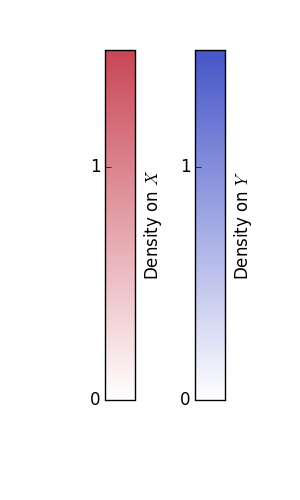
\includegraphics[clip,trim=0cm 0cm 0cm 0cm]{cmaps2d}
}
%\caption{\small{$F=0.05\times \TV$ }}
\end{subfigure}
\caption{Marginals of the optimal plan $\mathbf{R}$ for several unbalanced optimal transport problems (quadratic cost, divergence specified in the captions).}
\label{fig_2Dmarginals}
\end{figure}
%%%%%%%%%%%%%%%%%%%%%%%%%%%%%%%%%%%%%%%%%%%%%%%%%
\begin{figure}
 \centering
 %
\begin{subfigure}{0.24\linewidth} 
\centering
 \reflectbox{\rotatebox[origin=c]{180}{\resizebox{1.\linewidth}{!}{

\includegraphics[clip,trim=3cm 1cm 3cm 1cm]{map2d_OT}
}}}
\caption{$\iota_{\{=\}}$}
\end{subfigure}%
\begin{subfigure}{0.24\linewidth} 
\centering
 \reflectbox{\rotatebox[origin=c]{180}{\resizebox{1.\linewidth}{!}{

\includegraphics[clip,trim=3cm 1cm 3cm 1cm]{map2d_KLb}
}}}%
\caption{$0.1\times \KL$}
\end{subfigure}
\begin{subfigure}{0.24\linewidth} 
\centering
 \reflectbox{\rotatebox[origin=c]{180}{\resizebox{1.\linewidth}{!}{

\includegraphics[clip,trim=3cm 1cm 3cm 1cm]{map2d_RG}
}}}%
\caption{$\RG_{[0.7,\, 1.2]}$}
\end{subfigure}%
\begin{subfigure}{0.24\linewidth} 
\centering
 \reflectbox{\rotatebox[origin=c]{180}{\resizebox{1.\linewidth}{!}{

\includegraphics[clip,trim=3cm 1cm 3cm 1cm]{map2d_TV}
}}}
\caption{$0.05\times \TV$}
\end{subfigure}
\caption{Representation of the transport map for the experiments of Figure \ref{fig_2Dmarginals}. %Particles which are associated by the transport map are given identical colors.
}
\label{fig_2Dplans}
\end{figure}

%%%%%%%%%%%%%%%%%%%%%%%%%%%%%%%%%%%%%%%%%%%%%%%%%%
\paragraph{Color transfer.}
In general it is difficult to display optimal transport maps for three-dimensional problems. An interesting application which allows intuitive visualization is color transfer: a classical task in image processing where the goal is to impose the color histogram of one image onto another image. 
%
Optimal transport between histograms has proven useful for problems of this sort such as contrast adjustment~\cite{delon2006movie} and color transfer via 1D transportation~\cite{pitie2007automated}. Indeed, optimal transport produces a correspondence between histograms which minimizes the total amount of color ``distortion'' (where the notion of distortion is specified by the cost function) and thus maintains maximal visual consistency. 
%
%Some work has been done to tune this approach for instance by processing independently the luminance and the chrominance data or by building a specific model allowing for mass variation. 
%Although there is no quantitative metric to compare different methods, the use of novel generic unbalanced optimal transport for tackling the transport allows to obtain state of the art quality results in challenging cases (see Figure \ref{fig_colortransfer}) with a generic algorithm.
%
%The experiment on shows that the good computational properties of the proposed algorithm allows to perform transfer directly on the CIE-Lab (3 dimensional) color space (instead of subspaces as all previous works) and the flexibility on the marginal constraints allows to obtain good results by just applying the algorithm as is.
%fs source, ft target

In our experiments we represent colors in the three-dimensional ``CIE-Lab'' space (one coordinate for luminance and two for chrominance), resized to fit into a cuboid  $X=Y=[0,1]^3$, discretized into $I=J=64 \times 32 \times 32$ uniform bins and we choose the quadratic cost $c(x,y) = |x-y|^2$. The anisotropic dimensions of $X$ account for the fact that the eye is more sensitive to variations in luminance than variations in chrominance.

Let $\Omega \subset \RR^2$ be the image domain. An image is described by a function $g : \Omega \rightarrow X$ and its color histogram is the pushforward of the Lebesgue measure on $\Omega$ by $g$.
%Any color can be specified by three coordinates (e.g.\ $1$ for luminance and $2$ for chrominance in the ``CIE-Lab'' description). Thus an image can be described by a function $g$ which takes a point on the image plane $\Omega \subset \RR^d$ and returns a color in $\RR^3$. The color histogram is then the pushforward of the uniform measure on $\Omega$ by $g$.
%
%In our experiments, the domains $X=Y$ is the ``CIE-Lab'' color space, resized to fitted into a cuboid of dimension $[1.5 , 0.4, 0.4]$ discretized into $64\times32\times32$ uniform bins and $c$ is the quadratic cost $c(x,y)=|y-x|^2$ (the dimensions of $X$ account for the fact that the eye is more sensitive to variations in luminance than variations in chrominance).
Let $g_X : \Om \to X$ and $g_Y: \Om \to Y(=X)$ be two images and $p$, $q$ be the densities of the associated color histograms with respect to the reference measures $\mathbf{\d x} = \mathbf{\d y} = \ones_I$ which gives unit mass to each point of $X$. We run Algorithm \ref{algo_scaling_discrete} with the ``separable kernel'' method (see Section \ref{sec_implementation}) to obtain an (unbalanced) optimal transport plan $\mathbf{R}$.
%
An approximate transport map $T$ is then computed according to the barycentric projection (as already used for instance in~\cite{2015-solomon-siggraph})
\eq{
T(x_i)=\mathbf{T}_i \qwhereq
\mathbf{T} \eqdef (\mathbf{R}. \mathbf{y}^1,\mathbf{R}.\mathbf{y}^2,\mathbf{R}. \mathbf{y}^3)/\mathbf{R}. \ones_J
%T : (x^1,x^2,x^3) \mapsto \left(\frac{R(y\odot \d y)}{R.\d y}\right)_i
} %( this recovers the true transport map when the regularization parameter $\epsilon\to 0$). 
where $\mathbf{y}=(\mathbf{y}^1,\mathbf{y}^2,\mathbf{y}^3)\in \RR^{J\times 3}$ is the vector of coordinates of the points in $Y(=X)$. The modified image is finally obtained as $T\circ g_X$.

On Figure \ref{fig_colortransfer}, we display the color transfer between very dissimilar images, computed with parameter $\epsilon = 0.002$. The algorithm was stopped after $2000$ iterations and the running time was approximately $160$ seconds. This intentionally challenging example is insightful as it exhibits a strong effect of the choice of the divergence.
%
There are no quantitative measures for the quality of a transformed image, but the application of unbalanced optimal transport allows to select the ``right amount of colors'' in the target histogram so as to match the modes of the initial histogram and yields meaningful results.

\begin{figure}
 \centering
 %
 \begin{subfigure}{0.34\linewidth} 
\centering
 \resizebox{1.\linewidth}{!}{
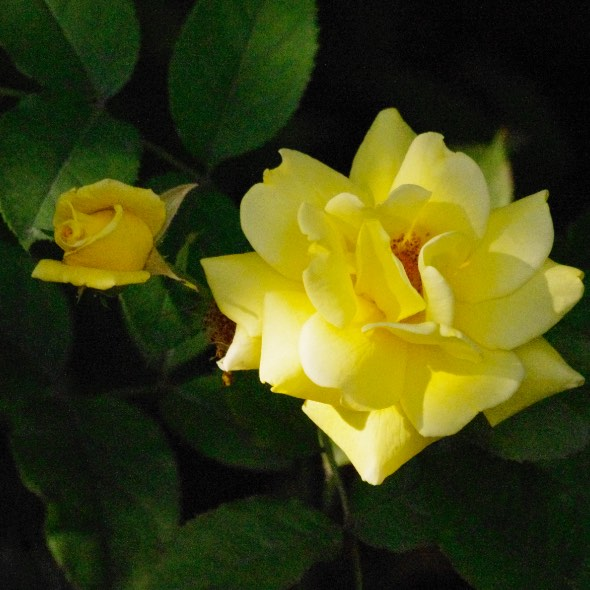
\includegraphics[clip,trim=0cm 0cm 0cm 0cm]{fleur}
}
\caption{Image $g_X$}
\end{subfigure}%
\quad
\begin{subfigure}{0.34\linewidth} 
\centering
 \resizebox{1.\linewidth}{!}{
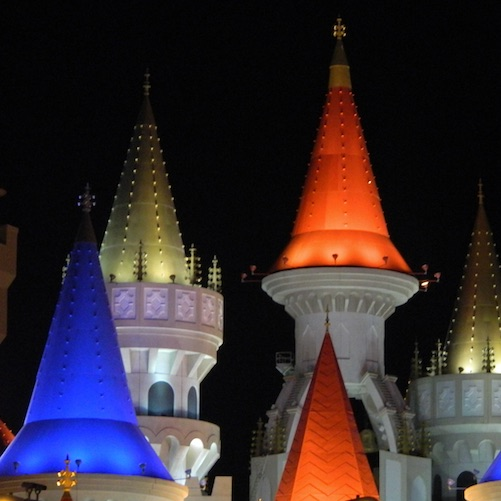
\includegraphics[clip,trim=0cm 0cm 0cm 0cm]{vegas}
}
\caption{Image $g_Y$}
\end{subfigure}
\hfill
\begin{subfigure}{0.24\linewidth} 
\centering
 \resizebox{1.\linewidth}{!}{
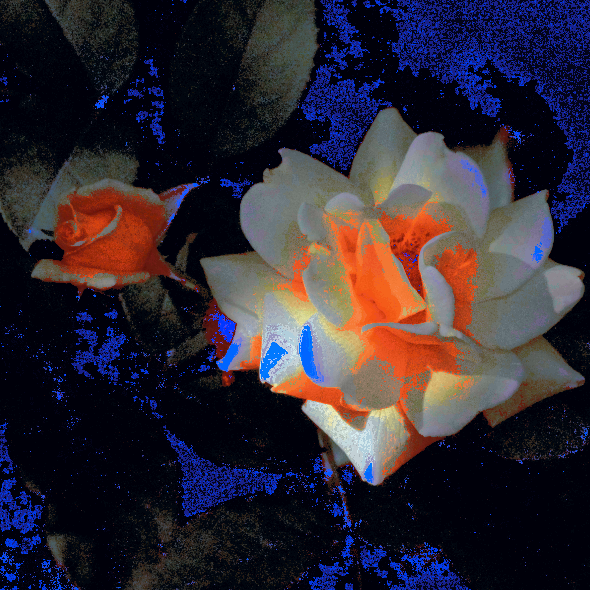
\includegraphics[clip,trim=0cm 0cm 0cm 0cm]{fleur_vegas_OT}
}
\caption{$\iota_{\{=\}}$}
\end{subfigure}%
\begin{subfigure}{0.24\linewidth} 
\centering
 \resizebox{1.\linewidth}{!}{
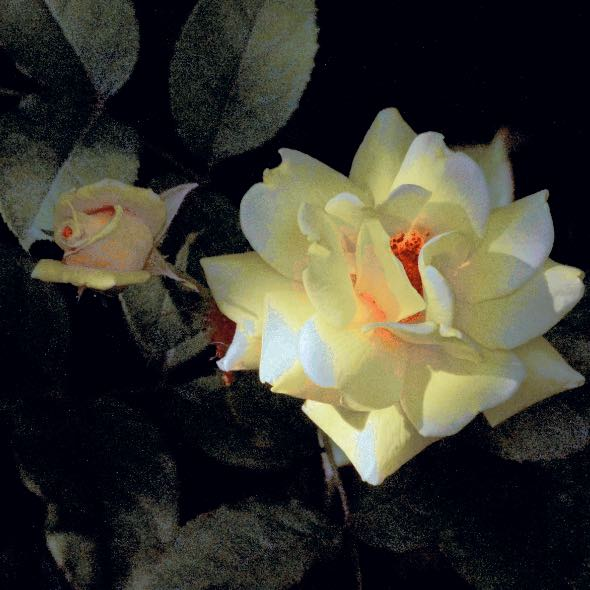
\includegraphics[clip,trim=0cm 0cm 0cm 0cm]{fleur_vegas_KL}
}
\caption{$0.03\times \KL$}
\end{subfigure}%
\begin{subfigure}{0.24\linewidth} 
\centering
 \resizebox{1.\linewidth}{!}{
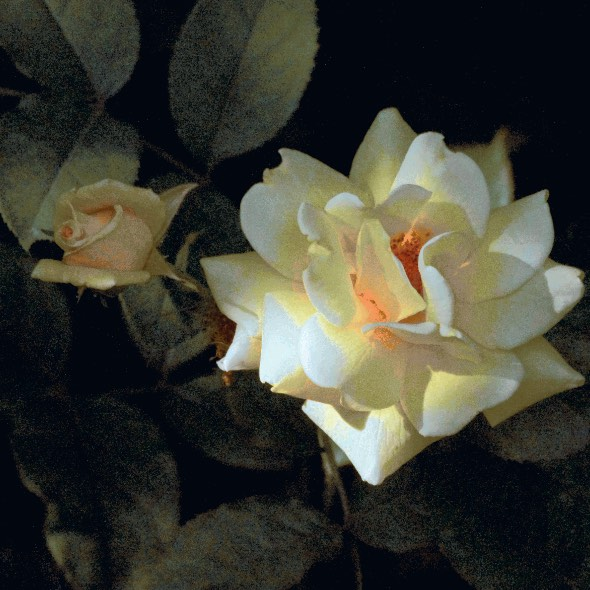
\includegraphics[clip,trim=0cm 0cm 0cm 0cm]{fleur_vegas_RG}
}
\caption{$\RG_{[0, \, 5]}$}
\end{subfigure}%
\begin{subfigure}{0.24\linewidth} 
\centering
 \resizebox{1.\linewidth}{!}{
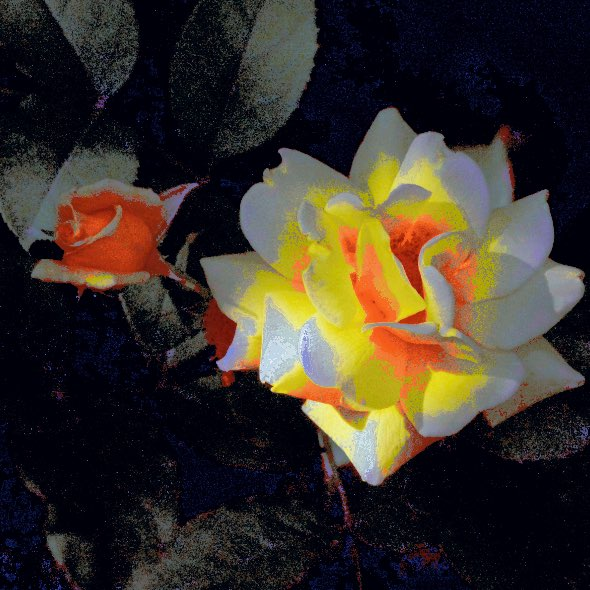
\includegraphics[clip,trim=0cm 0cm 0cm 0cm]{fleur_vegas_TV}
}
\caption{$0.2\times \TV$}\label{subfig:colorTV}
\end{subfigure}%
\caption{A challenging color transfer experiment where the colors of the image $g_Y$ are transferred to the image $g_X$. In all cases $F_1=\iota_{\{=\}}(\cdot\,|\,p)$ and $F_2$ is the divergence with respect to $q$ specified in the caption. Note that on Figure \ref{subfig:colorTV} some colors do not ``move''. The parameters for $F_{2}$ are chosen arbitrarily.}
\label{fig_colortransfer}
\end{figure}
